\subsection*{\lr{2.3.1} \quad (رابطهٔ بین \lr{$\leftrightarrow$} و \lr{$\equiv$})}
    عملگر «معادل» (\lr{$\leftrightarrow$}) یک \emph{عملگر بولی} در منطق گزاره‌ای است و می‌تواند در فرمول‌های این منطق ظاهر شود. اما «معادل منطقی» (\lr{$\equiv$}) یک عملگر بولی نیست؛ بلکه نشانه‌ای برای ویژگی یک جفت فرمول در منطق گزاره‌ای است. این دو مفهوم می‌توانند سردرگمی ایجاد کنند، زیرا ما از واژگان مشابه هم برای زبان مَحْتوایی (در اینجا زبان منطق گزاره‌ای) و هم برای زبان مَدرِکی—آنچه برای استدلال دربارهٔ زبان محتوا استفاده می‌کنیم—بهره می‌بریم.
    
    با این حال، معادل بودن (\lr{$\leftrightarrow$}) و معادل منطقی (\lr{$\equiv$}) ارتباط نزدیکی دارند، چنان‌که در قضیهٔ زیر نشان داده شده است:
    
    \begin{theorem}[قضیه \lr{2.29}]
      $A_1 \equiv A_2$ اگر و تنها اگر $A_1 \leftrightarrow A_2$ در هر تعبیر صدق کند.
    \end{theorem}
    
    \begin{proof}
      فرض کنید $A_1 \equiv A_2$ و $\mathscr{I}$ یک تعبیر دلخواه باشد. از تعریف معادل منطقی می‌دانیم:
      \[
      v_{\mathscr{I}}(A_1) = v_{\mathscr{I}}(A_2).
      \]
      طبق جدول ارزش صدق (شکل \lr{2.3})، در این صورت داریم:
      \[
      v_{\mathscr{I}}(A_1 \leftrightarrow A_2) = T.
      \]
      از آنجا که $\mathscr{I}$ دلخواه بود، نتیجه می‌شود $A_1 \leftrightarrow A_2$ در همهٔ تعبیرها درست است.
      
      اثبات جهت معکوس (یعنی اگر $A_1 \leftrightarrow A_2$ در همهٔ تعبیرها درست باشد، آنگاه $A_1 \equiv A_2$) به‌صورتی مشابه انجام می‌پذیرد.
    \end{proof}
    
    \begin{figure}[ht]
      \centering
      \begin{latin}
      \resizebox{0.7\textwidth}{!}{
      \begin{tikzpicture}[
        level distance=1.5cm,
        sibling distance=4cm,
        level 2/.style={sibling distance=2cm},
        level 3/.style={sibling distance=1cm},
        edge from parent path={(\tikzparentnode.south) -- (\tikzchildnode.north)}
      ]
      \node {$\leftrightarrow$}
        child { 
          node {$\rightarrow$}
          child {node {$p$}}
          child {node {$p$}}
        }
        child { 
          node {$\rightarrow$}
          child {
            node {$\neg$}
            child {node {$p$}}
          }
          child {
            node {$\neg$}
            child {node {$q$}}
          }
        };
      \end{tikzpicture}
      }
      \\
      \resizebox{0.2\textwidth}{!}{
        \begin{tikzpicture}[
          level distance=0.75cm,
          sibling distance=0.75cm,
          level 2/.style={sibling distance=1cm},
          edge from parent path={(\tikzparentnode.south) -- (\tikzchildnode.north)}
        ]
        \node {$\rightarrow$}
          child { 
            child {node {$p$}}
            child {node {$p$}}
          };
        \end{tikzpicture}
      }
      \hfill
      \resizebox{0.1\textwidth}{!}{
        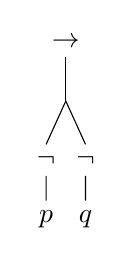
\begin{tikzpicture}[
          level distance=0.75cm,
          sibling distance=0.75cm,
          level 2/.style={sibling distance=0.5cm},
          level 3/.style={sibling distance=0.5cm},
          edge from parent path={(\tikzparentnode.south) -- (\tikzchildnode.north)}
        ]
        \node {$\rightarrow$}
          child { 
            child {
              node {$\neg$}
              child {node {$p$}}
            }
            child {
              node {$\neg$}
              child {node {$q$}}
            }
          };
        \end{tikzpicture}
      }
      \hfill
      \resizebox{0.1\textwidth}{!}{
        \begin{tikzpicture}[
          level distance=0.75cm,
          sibling distance=0.75cm,
          level 2/.style={sibling distance=0.5cm},
          level 3/.style={sibling distance=0.5cm},
          edge from parent path={(\tikzparentnode.south) -- (\tikzchildnode.north)}
        ]
        \node {$\neg$}
          child { 
            child { node {$p$} }
          };
          
        \end{tikzpicture}
      }
      \hfill
      \resizebox{0.1\textwidth}{!}{
        \begin{tikzpicture}[
          level distance=0.75cm,
          sibling distance=0.75cm,
          level 2/.style={sibling distance=0.5cm},
          level 3/.style={sibling distance=0.5cm},
          edge from parent path={(\tikzparentnode.south) -- (\tikzchildnode.north)}
        ]
        \node {$\neg$}
          child { 
            child { node {$q$} }
          };
          
        \end{tikzpicture}
      }
      \hfill
      \resizebox{0.1\textwidth}{!}{
        \begin{tikzpicture}[
          level distance=0.75cm,
          sibling distance=0.75cm,
          level 2/.style={sibling distance=0.5cm},
          level 3/.style={sibling distance=0.5cm},
          edge from parent path={(\tikzparentnode.south) -- (\tikzchildnode.north)}
        ]
        \node {$p$};
          
        \end{tikzpicture}
      }
      \hfill
      \resizebox{0.1\textwidth}{!}{
        \begin{tikzpicture}[
          level distance=0.75cm,
          sibling distance=0.75cm,
          level 2/.style={sibling distance=0.5cm},
          level 3/.style={sibling distance=0.5cm},
          edge from parent path={(\tikzparentnode.south) -- (\tikzchildnode.north)}
        ]
        \node {$q$};
          
        \end{tikzpicture}
      }
      \end{latin}
      \renewcommand{\thefigure}{\lr{2.4}}
      \caption{زیر فرمول ها}
      \end{figure}